% Based on the ACM SIG Proceedings sample. The KDD Research CFP specifies
% sigconf,anonymous,review. Overleaf root document: main.tex.
% The original vector overview is PDF 1.7.
\ifdefined\pdfminorversion\pdfminorversion=7\relax\fi
\documentclass[sigconf,anonymous,review]{acmart}
\setcopyright{none}
\acmDOI{}
\acmISBN{}
\acmConference[KDD 2027 Research Track]{KDD 2027 Research Track}{August 2027}{San Jose, CA, USA}
\acmBooktitle{Manuscript prepared for the KDD 2027 Research Track}
\acmYear{2027}
\usepackage{amsmath}

\begin{document}
\title[Which Analyses Can Agent-Generated Cohorts Support?]{Which Scientific Analyses Can Agent-Gener\-ated Biomedical Cohorts Support?}
\author{Anonymous Author(s)}

\begin{abstract}
A published table can determine the odds ratio for two biomarker thresholds while leaving their continuous association open. We ask a scientific agent to read a study, choose a joint model and write a sampler. We apply the same estimator to its virtual records and to measured cohorts, tracing each result to a source statistic or a modeling choice. Seven iron-status models that met the same source checks gave threshold odds ratios of 6.55--6.86 and rank correlations from $-0.272$ to $0.446$. In a separate Chinese community holdout, source counts implied an odds ratio of 5.08. Six agents produced continuous correlations of 0.293--0.320 against a measured 0.317. Retrospectively re-pairing the same values within hemoglobin bands preserved all four threshold counts and reduced expected correlations to 0.244--0.249. We then prospectively compared six fresh agents and a statistical generator allowed to fit within-band dependence. With the same Chinese evidence and identical marginal values, all six agents chose the same copula family as the comparator. In 603 Nigerian mothers, measured rank correlation was 0.010 (95\% interval $-0.064$ to 0.086), compared with 0.308 for the agents and 0.303 for the comparator. The within-survey result localized the contribution of pairing. The external test showed the limits of carrying that relationship into another population.
\end{abstract}

\ccsdesc[500]{Computing methodologies~Modeling and simulation}
\ccsdesc[300]{Applied computing~Life and medical sciences}
\keywords{scientific agents, synthetic biomedical data, joint distributions, evidence synthesis, analysis utility}
\maketitle

\begin{figure*}[t]
\centering
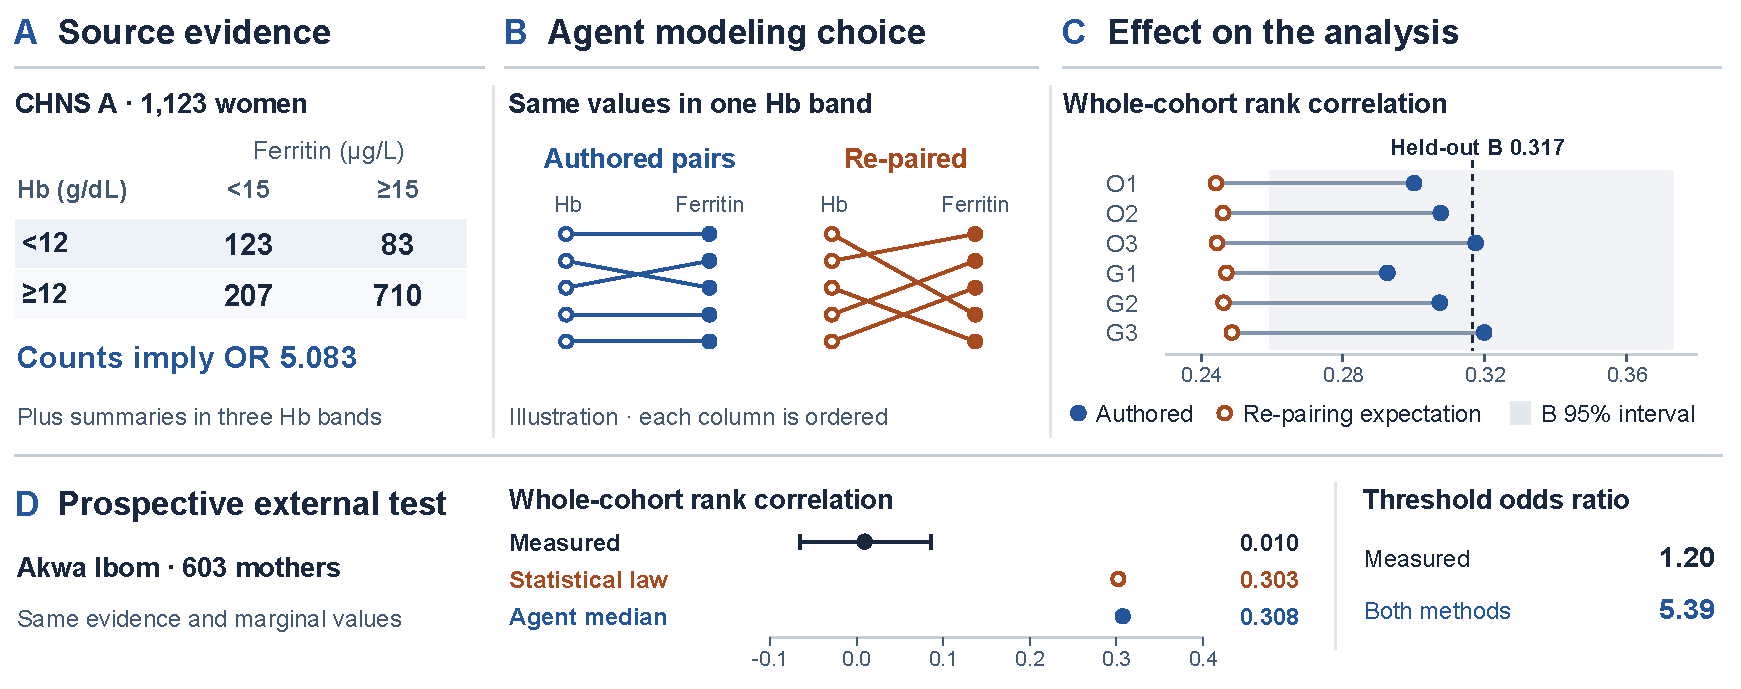
\includegraphics[width=\textwidth]{figures/evidence-and-pairing.pdf}
\caption{Where a generated association comes from. (A) Four counts in the CHNS A evidence communities determine the threshold odds ratio. (B) Two illustrative pairings use the same five values of each biomarker within one hemoglobin (Hb) band. (C) Six original-evidence models and their random re-pairing expectations are compared with held-out CHNS B. O1--O3 are ordinary constructors and G1--G3 are workflow-guided. Re-pairing preserves each model's threshold counts. We specified this check after disclosure. (D) A separate prospective experiment supplies the same evidence, including a middle-band contrast, and the same virtual marginal values to fresh agents and a statistical generator that allows within-band dependence. The bar is the Nigerian measured rank's cluster-bootstrap 95\% interval.}
\Description{Four source counts imply a threshold odds ratio of 5.083. Two small diagrams pair the same values differently. In Chinese held-out communities, the authored ranks of 0.293 to 0.320 approach the measured 0.317. In Nigeria, the measured rank is 0.010 and both virtual approaches give about 0.30. The measured threshold odds ratio is 1.20, versus 5.39 for both methods.}
\label{fig:method}
\end{figure*}

\section{Introduction}
A study in rural northern China reports anemia counts across eight combinations of iron, folate and vitamin B$_{12}$ status~\cite{zhu}. A researcher with no access to those individual records wants a virtual cohort of US women. She intends to use the same records for two questions. How much higher are the odds of anemia among women with low ferritin? How closely do hemoglobin and ferritin track each other across their continuous ranges? An agent can answer the first question \emph{for the source study} by collapsing the eight rows into four cells. Any assignment of continuous measurements within those cells preserves that answer. Many such assignments give different answers to the second question. Moving from the Chinese study to the US population introduces a further uncertainty, even for the first question.

This example motivates an evaluation of scientific agents in which the deliverable is a dataset. A researcher specifies a population, measurements and intended analyses. The agent reads the evidence, chooses how to model the relationships that the publications leave open, and delivers a program that can draw complete records. The researcher can then run regressions, compare subgroups or apply screening rules. These are concrete uses when records are costly to collect or unavailable. Their value depends on the analysis one plans to perform.

Previous work has shown how to generate synthetic cohorts using shared fitted models, aggregate tabulations, trial curves and published covariates~\cite{filshtein,llmsynthor,synthipd,kmgen}. Our question concerns the point where scientific modeling discretion enters this process. Two agents can reproduce the same table by writing different sampling laws. A single law can reproduce a regression slope and miss the dependence that governs a screening rule. We therefore evaluate one \emph{analysis in one population} at a time. We keep the analysis code fixed when changing its input and trace the resulting estimate back to the article and the authored program.

Our contributions concern three questions about the use of agent-generated records (Figure~\ref{fig:method}).
\begin{enumerate}
\item \textbf{What can a reader trace to the article?} We follow an agent's construction from the reported numbers and their algebraic implications through the joint law it chose and the sampler it wrote. We then apply the same analysis code to the resulting records and to a measured cohort.
\item \textbf{Which answers survive a change of law?} We compare alternative pressure and iron models under common source constraints. Seven iron models reproduce similar threshold odds while permitting continuous associations of different signs.
\item \textbf{What difference does the agent's pairing make?} On a community holdout we test two prespecified group analyses. A retrospective re-pairing of each model's records isolates the contribution of its within-band dependence. A prospective comparison in Nigeria gives the agent and a statistical generator the same source material and virtual biomarker values. Only their pairing rules differ.
\end{enumerate}

\section{From a research request to executable records}
\label{sec:method}



\paragraph{Scientific contract.}
A request names the unit of observation, population, measurement units and intended analyses. For example, the iron request calls for continuous hemoglobin and ferritin in nonpregnant US women aged 20--44. We disclose the analyses to the constructor so it can seek appropriate evidence. The measured target records and their analysis results stay with the evaluator. All experiments here generate whole records. Figure~\ref{fig:method} follows one such construction from its source counts to two group analyses. In the community holdout, constructors also see tables newly calculated in the evidence communities. Individual measurements from either half remain unavailable to them.

Write $s_j(P_j)$ for a statistic evaluated under the population, measurement and adjustment rules of source study $j$. A paper reports a rounded estimate of this quantity. The researcher's question is an analysis $a(P_T)$ in target population $T$. Even exact knowledge of $s_j(P_j)$ generally leaves open both the shape of the source distribution and the correspondence between $P_j$ and $P_T$. We use this distinction in two ways. We compare a generated estimate of $a$ with the same estimate in a measured sample. Where source summaries permit several laws, we can also ask whether varying the law changes $a$ while preserving those summaries.

\paragraph{Agent and execution service.}
In the initial original-paper experiments (Section~\ref{sec:original}), each fresh model session received a starting paper, the request, tools for reading and supplementary retrieval, an output schema and an execution budget. The agent could inspect source tables and methods, resolve units, propose a dependence structure, and choose numerical parameters. It returned an executable sampler, its parameters and a record of consequential choices. It could inspect a trial draw and submit a revision. The execution service validated the interface, ran the submitted program in isolation and recorded its identity and seeds. The coordinator supplied the task and starting article. The constructor selected the scientific law. The final rows were sampled from that law. The study therefore tests authorship of a reusable generator from an assigned paper. Each of the two articles was assigned to three sessions.

\paragraph{Audit of a modeling decision.}
For each quantity we record what the source reported, how the agent transformed it and how the code used it. We separately record any change of population or statistical definition. For example, a partial correlation can be exactly derived from a source matrix while its use as a residual correlation after additional adjustment remains an assumption. We check the submitted program against the account of the model choice and independently recompute scientific estimates. This audit can establish that a model implements its stated choice. Only evidence on the requested analysis can establish how useful that choice was.

\paragraph{Evaluation.}
Each constructor commits its program before the final draws. Draws with different seeds measure variation conditional on that program. Separate constructors can express different modeling choices. For each task we run a single estimator implementation on generated records and the measured reference under the relevant sampling design. For the published lifestyle analysis, this is a reimplementation of the reported regression. A reference value estimates a quantity in a measured sample and carries uncertainty. The community holdout specifies planning tolerances and a minimum worthwhile change before generation. Elsewhere we report discrepancies in native units. All scores here describe group analyses. We did not evaluate individual-level prediction.

\section{Can the agent model what the paper reports?}
\label{sec:original}

\begin{figure*}[t]
\centering
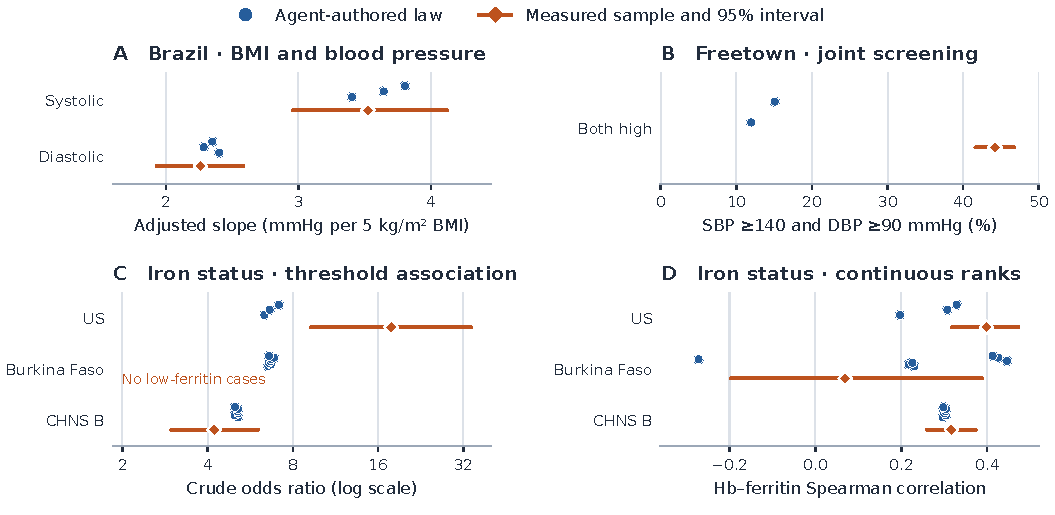
\includegraphics[width=.98\textwidth]{figures/analysis-support.pdf}
\caption{What the virtual cohorts support when the scientific analysis stays fixed. Each circle is one agent-authored law. Diamonds and bars show measured estimates and their 95\% intervals. (A) Three constructors recover the scale of the adjusted Brazilian blood-pressure slopes. (B) Two laws that share five source moments both understate the joint screening rate in the deposited Freetown fields. (C, D) Each iron cohort supplies both a threshold odds ratio and a continuous rank correlation. Burkina Faso has no low-ferritin cases. In CHNS the six final laws meet both prespecified planning tolerances. Brazil and the US are development comparisons. Freetown and Burkina Faso are external assessments. CHNS B comprises communities held out within a survey. The Brazilian bars describe row-resampling stability.}
\Description{Four panels compare modeled and measured quantities in their native units. Blood-pressure slopes are close in Brazil. The Freetown joint rate is much higher in the release. Iron models preserve the source odds ratio in the US and Burkina Faso tasks while continuous ranks vary. Both CHNS analyses show positive associations near the held-out estimates.}
\label{fig:support}
\end{figure*}
We ran three fresh sessions on each of two requests using the same recorded GPT configuration. All six located the relevant table in the assigned original article, performed a numerical derivation, authored a whole-cohort generator, inspected one simulated trial and retained the first candidate. Each law produced three final draws. The 18 tables contain 72,000 simulated records. Independent computation reproduced all 99 draw-level analysis and diagnostic estimates to within $7.6\times10^{-14}$. Construction used 142 model calls at an estimated token tariff of US\$1.51. These counts describe six modeling decisions.


\paragraph{Blood pressure.}
The assigned article studied partnered adults aged at least 40 in rural Burkina Faso~\cite{jaspert}. Its correlation matrix gives the associations of age, body mass index (BMI), systolic blood pressure (SBP) and diastolic blood pressure (DBP). Each agent combined its entries to obtain the source age- and BMI-adjusted residual correlation, approximately 0.788. The source also reports BMI regression coefficients from a more extensively adjusted model. The agents used positive diastolic and pulse pressures and summed them to obtain systolic pressure. They chose different demographic distributions and conditional pressure levels. This construction enforces the physical ordering of the two pressures for every draw.

We applied the target regressions to virtual records and compared them with estimates from 8,352 eligible participants in the Brazilian National Health Survey (PNS)~\cite{pns}. The age- and sex-adjusted systolic slope ranged from 3.40 to 3.80 mmHg per five BMI units, bracketing the measured 3.52. The corresponding diastolic slopes were 2.29--2.40 versus 2.26. The pressure correlation after adjusting for age, sex and BMI was 0.772--0.781 versus 0.717. All three laws also yielded wider pressure distributions than the measured sample (Appendix~\ref{app:profiles}). Thus a user could recover the direction and approximate scale of these BMI associations while overestimating dependence between the paired measurements.

\paragraph{Iron status.}
Of the women in the source table, 173 had both markers low, 85 had only low hemoglobin, 331 had only low ferritin and 1,082 had neither~\cite{zhu}. Each agent computed the crude odds ratio, $(173\times1082)/(85\times331)=6.65$, and distinguished it from the paper's adjusted odds ratio of 6.448. One agent then used a Clayton copula to couple continuous biomarker values. Another modeled two latent iron-store components and a change in hemoglobin response below a threshold. The third used a saturating response with inflammatory and other-anemia components. Supplementary evidence informed marginal assumptions. All three authors noted an ambiguity in the source's ferritin labeling.

We evaluated crude threshold odds, joint prevalence and rank correlation against survey-weighted US National Health and Nutrition Examination Survey (NHANES) estimates from 979 eligible women~\cite{nhanes}. The thresholds were hemoglobin $<12$ g/dL and ferritin $<15$ $\mu$g/L. Generated odds ratios were 6.35--7.14, close to the source's 6.65. The measured US odds ratio was 17.79. All three programs preserved a positive association and substantially understated its strength in this comparison. For the same records, the prevalence of both low markers was 4.67--5.85\% versus 7.63\%, and Spearman correlation ranged from 0.197 to 0.329 versus 0.398 (Figure~\ref{fig:original}). A correct table extraction can therefore coexist with appreciable error after population transfer.

\paragraph{What does direct arithmetic already give the researcher?}
Five times the published BMI coefficients gives 3.75 mmHg for SBP and 2.20 mmHg for DBP in the source's fully adjusted model. Those two numbers provide informative comparisons with the Brazilian slopes, even before simulation. Likewise, the four iron counts yield the crude odds ratio and a joint-low prevalence of 10.35\% for the Chinese study. They supply no continuous rank correlation. For that question, choosing how to populate the four cells with continuous values is the scientific modeling step. Comparing the three authored programs makes that choice visible.

\section{What changes when the agent gets joint evidence?}
\label{sec:controlled}
We held the research request and modeling interface fixed within each task and changed the supplied evidence. Three fresh constructors worked in each of three conditions per case, with three final seeds per constructor. The first condition provided the common base. For pressure, this already contained previously published relationship evidence. For iron status, it supplied study context. The second condition added single-variable summaries from the selected source. The third added a joint block \emph{from the same source sample}. This consisted of six pairwise correlations for pressure, or the paired low-marker counts for iron. The latter two conditions differed only in that block. No target feedback or programmed numerical relationship entered these comparisons.

\begin{table}[t]
\caption{Mean absolute discrepancy by evidence condition. The last two columns differ only in the joint source block. Lower is closer to the measured sample within each row.}
\label{tab:evidence}
\centering
\begin{tabular}{@{}lrrr@{}}
\toprule
Requested analysis & Base & Marginal & Joint\\
\midrule
BP residual correlation & .1632 & .1633 & \textbf{.0350}\\
BMI--SBP slope & .1934 & .3396 & .5091\\
BMI--DBP slope & .7276 & .7378 & .7550\\
Iron log odds ratio & 1.5495 & 1.7620 & \textbf{.9373}\\
Both markers low (pp) & 1.7903 & .5187 & 2.5940\\
Iron rank correlation & .0769 & .0447 & .1736\\
\bottomrule
\end{tabular}
\end{table}

Table~\ref{tab:evidence} reports discrepancies for every requested analysis. We computed the absolute error for each draw and averaged first across seeds, then equally across constructors. The two pressure slopes are in mmHg per five BMI units. The iron odds ratio is evaluated on the natural-log scale. Adding the matrix reduced residual-correlation error from 0.1633 to 0.0350. Adding the four-cell table reduced log-odds-ratio error from 1.7620 to 0.9373. The two other pressure estimates and the two other iron estimates moved farther from their respective sample references. In particular, the joint table identifies a threshold association in its source sample but gives neither the target prevalence nor the within-cell ordering needed for continuous ranks. These results identify the change across the tested evidence conditions. Their magnitude is descriptive across three constructors per condition.

\section{Can the same pressure moments predict joint screening?}
\label{sec:prospective}
Before inspecting paired outcome values in a new Freetown screening release~\cite{freetown,freetowndata}, we specified two analyses: the unadjusted Pearson correlation of SBP and DBP, and the fraction simultaneously reaching 140 mmHg systolic \emph{and} 90 mmHg diastolic. The latter is a conjunction of two thresholds. It has a different interpretation from a clinical hypertension diagnosis. The agent received five rounded source summaries from the rural Burkina Faso study~\cite{jaspert}, comprising means 125.22 and 80.54 mmHg, standard deviations 18.22 and 10.98 mmHg, and raw correlation 0.78. It also received the target sampling context. This experiment starts from extracted summaries. The earlier experiments in Section~\ref{sec:original} test original-paper reading.


One fresh agent was asked to propose a primary and an alternative law and state which analyses the source constrained. Before disclosure, it identified the correlation as reported, the joint threshold as underdetermined and the application to a new population as uncertain. Its primary model coupled positive DBP and pulse pressure with a bivariate lognormal law. A statistical comparator specified in advance from the same five numbers independently used this family. The agent's alternative was a 75:25 mixture. It separated the component means and subtracted their between-component contribution from the within-component covariance. These are hypothetical population structures. Both laws preserve all five working moments, including an exact population correlation of 0.780.

Independent numerical integration of the fixed programs gave joint threshold probabilities of 11.9449\% and 15.0851\%. These two examples establish a 3.14 percentage-point difference consistent with the five summaries. They give a lower bound on the range of answers permitted by those constraints. The full range may be wider. A separately prespecified finite-draw criterion asked whether the simulated gap, after subtracting four times the sum of Monte Carlo standard errors, exceeded two percentage points. The adjusted gap was 1.60 points, below the criterion. We report both results because they answer different questions.

After the freeze we analyzed the deposited fields of 1,244 eligible screening participants aged 40 or older. Their correlation was 0.859 (within-zone bootstrap 95\% interval 0.847--0.872), and 44.21\% met both thresholds (41.64--46.79\%). All three simulated arms were far below the released joint rate (Figure~\ref{fig:support}B and Appendix Figure~\ref{fig:freetown}). A post-disclosure count clarified how to interpret that difference. Of the eligible records, 550 met both thresholds, 694 met neither, and neither isolated exceedance occurred. The same pattern held across all 2,394 released records. The codebook identifies the component fields as added variables. Their pairing history remains unresolved. The measured discrepancy applies to the deposited fields. The unresolved pairing limits its biological interpretation.


\section{Which iron analyses survive a change of model?}
\label{sec:ironpros}
We repeated the prospective test from the full Chinese iron-status article~\cite{zhu}. This time the target was adult nonpregnant, nonlactating mothers in rural Burkina Faso~\cite{burkina_iron}. Three fresh GPT sessions each submitted a primary generator. For each primary, two further sessions received the same article, research request and sealed program. One was asked for a second defensible model. The other was asked for a model that would expose the sensitivity of a requested analysis. A fixed statistical comparator independently sampled within the published categories. All constructors could see the scientific questions. The Burkina Faso measurements stayed with the evaluator.

The paper also reports ferritin geometric means and depletion frequencies across three hemoglobin bands. All three primary authors extracted the four crude counts correctly. All seven completed authors predicted that the source odds ratio was determined and that the rank correlation was sensitive. After a documented parameter-interface correction, the seven laws passed all 16 prespecified source checks (Appendix~\ref{app:ironpros}). Across the same virtual records, the odds ratio stayed near 6.65, while choices about ordering people within hemoglobin bands changed the continuous correlation. Four of six planned primary--alternative pairs completed. In all four, the rank gap exceeded its estimated simulation noise. Only one primary yielded both alternatives, which limits the prompt comparison.


For one parent the ordinary alternative changed the rank correlation from $0.217$ to $-0.272$. Its author chose a within-band Gaussian copula parameter of $-0.75$, an explicit sensitivity assumption with no measured support in the source. Two positive-dependence alternatives for another parent moved its correlation from $0.226$ to $0.426$ and $0.413$. Even the positive scenarios gave different effect sizes. Appendix~\ref{app:ironproof} shows why this freedom survives the group summaries.

After all draws and source checks were sealed, 44 women had complete paired measurements across 23 villages. The measured survey-weighted rank correlation was 0.069 (95\% village-bootstrap interval $-0.198$ to $0.389$). No participant met the ferritin threshold, and 18 met the hemoglobin threshold. The external odds ratio was unestimable. Both thresholds agreed with the release's own flags in all 44 records. Figure~\ref{fig:support}C--D compares these analyses across populations. Appendix Figure~\ref{fig:ironpros} identifies the individual laws. The source odds ratio was reproducible, several continuous relationships remained possible, and the new sample distinguished them imprecisely.

\section{Can the same virtual cohort support two held-out iron analyses?}
\label{sec:chns}
The external Burkina Faso sample had too few low-ferritin observations to evaluate the threshold analysis. For a test with information from the target population, we used the 2009 China Health and Nutrition Survey (CHNS)~\cite{chnsbio,chnsind}. We split whole communities within nine provinces before scoring. The evidence half (A) comprised 1,123 women in 110 communities. The held-out half (B) comprised 1,082 women in 107 other communities. All were aged 18--49 with paired central hemoglobin (Hb) and serum ferritin measurements. The halves shared no people, households or communities. The survey family had been used in development. The partition and its iron endpoint were new.

\paragraph{An identical starting point for each pair of revisions.}
Three ordinary coding agents and three agents given scientific modeling guidance used the same GPT configuration. Each received the Zhu article and two tables newly computed from A, one reporting joint threshold counts and the other summarizing ferritin by Hb band. Each chose its own law and parameters. Two further sessions independently reviewed each sealed law with the same feedback on its generated records and the original evidence. Only one received a new A statistic. Within Hb 12--$<14$ g/dL, geometric mean ferritin was 1.215 times as high at Hb 13--$<14$ as at 12--$<13$ g/dL (95\% interval 1.061--1.398). Neither branch received a whole-cohort rank correlation. We sealed all programs and outputs before opening B.

\paragraph{Final utility on the two prespecified analyses.}
We ran the same unweighted rank and threshold estimators on virtual and measured records. B's Spearman correlation was 0.317 (95\% community-bootstrap interval 0.259--0.373). All six augmented laws gave 0.297--0.304, within the prespecified absolute tolerance of 0.10. For low Hb ($<12$ g/dL) comparing low ferritin ($<15$ $\mu$g/L) with higher ferritin, the six crude odds ratios were 4.990--5.124. B's estimate was 4.218 (2.979--6.042). All six preserved the positive threshold association and met the factor-of-1.50 tolerance, while overstating its magnitude by 18--22\%. The A threshold table already implied an odds ratio of 5.083. The global rank analysis tests a relationship absent from the supplied tables. Both conclusions concern planning with these measured populations.

\begin{table*}[t]
\caption{What did the CHNS A evidence alone supply? The B reference is a Spearman correlation of 0.3168 and a crude odds ratio of 4.218. All four rows use only the original evidence. The retrospective statistical model and each of the six agent models use 36,000 draws per law. Ranges cover the six original-evidence agents. Re-pairing gives the expected correlation under a uniform permutation within each Hb band and leaves each agent's four threshold counts unchanged.}
\label{tab:chnsattribution}
\centering
\begin{tabular}{@{}lrrrr@{}}
\toprule
 & \multicolumn{2}{c}{Continuous Hb and ferritin} & \multicolumn{2}{c}{Threshold association}\\
\cmidrule(lr){2-3}\cmidrule(l){4-5}
Construction & Spearman $\rho$ & $|\rho-\rho_B|$ & Odds ratio & $|\log(\mathrm{OR}/\mathrm{OR}_B)|$\\
\midrule
Direct A threshold counts & --- & --- & 5.083 & 0.187\\
Statistical model, independent within Hb band & 0.2370 & 0.0798 & 5.023 & 0.175\\
Agent records, expected after within-band re-pairing & 0.2444--0.2489 & 0.0679--0.0724 & 4.998--5.175 & 0.170--0.205\\
Agent records, original pairing & 0.2927--0.3201 & 0.0008--0.0241 & 4.998--5.175 & 0.170--0.205\\
\bottomrule
\end{tabular}
\end{table*}

\paragraph{What does the agent add to the original evidence?}
After B was disclosed, we specified one statistical comparator that fits the A band sizes, Hb moments, ferritin geometric moments and depletion frequencies. It draws Hb and ferritin independently within each of the three reported Hb bands (Appendix~\ref{app:chnsstat}). It met both original target-comparison margins. Its pooled rank was 0.2370 (analytic population value 0.2414). All six original-evidence agent laws gave ranks closer to B (Table~\ref{tab:chnsattribution}). To isolate the contribution of pairing while keeping each agent's own bandwise marginals, we computed its expected rank after randomly re-pairing the two biomarkers within each band. Restoring the authored pairs reduced absolute rank error for all six, by a median of 0.0612. The threshold odds ratio was exactly invariant to this change. This localizes the improvement to an aspect of the model the A tables leave open. Its size is relative to the measured estimate on this split.

\begin{figure*}[t]
\centering
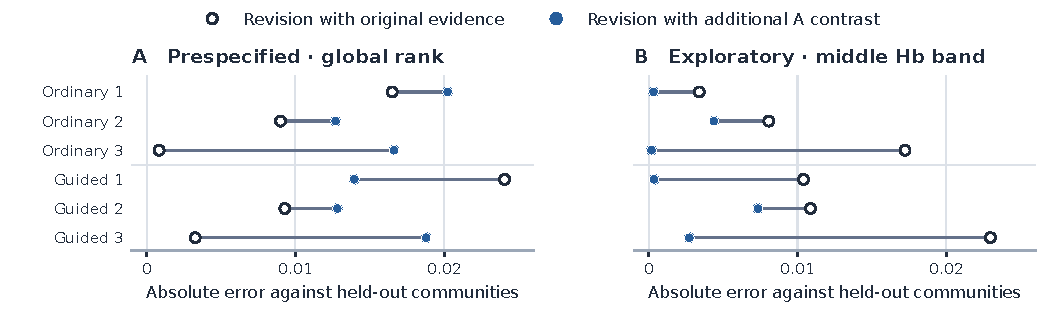
\includegraphics[width=.98\textwidth]{figures/chns-revision.pdf}
\caption{What changed when a constructor received one extra conditional contrast? Each row pairs two revisions of the same parent. Leftward movement means smaller absolute error against CHNS B. (A) On the prespecified whole-cohort rank correlation, one of six moves closer. (B) In a post hoc decomposition, all six move closer on the middle Hb band's weighted contribution to the global correlation. The two panels use the same scale. The B reference is a sample estimate.}
\Description{Paired error plots for three ordinary and three workflow constructors. Additional evidence lowers whole-cohort rank error for the first workflow constructor. It reduces the error in the middle-band contribution for every constructor.}
\label{fig:revision}
\end{figure*}

\paragraph{Incremental effect on the prespecified whole-cohort analysis.}
The revisions using only the original evidence reproduced all 18 initial tables byte for byte at the three shared seeds. Five of six augmented laws came closer to the supplied A contrast on the log scale. In B only one came closer on whole-cohort rank correlation (Figure~\ref{fig:revision}A). Median reductions in absolute rank error were $-0.0037$ for ordinary and $-0.0035$ for guided constructors. The prespecified material gain was 0.05. The largest control error against B was 0.024, already below that benchmark. Even a perfect revision at the observed B estimate could therefore have gained at most 0.024.

\paragraph{Exploratory explanation of the local change.}
After opening B, we partitioned the covariance of standardized global midranks by Hb band. The middle band's probability-weighted within-band contribution to the whole-cohort correlation was 0.03429. All six augmented laws estimated this particular component more closely (Figure~\ref{fig:revision}B). Its median absolute error fell from 0.01064 to 0.00155. The between-band component was larger, 0.27054 in B, and stayed near 0.24--0.25 in both revisions. Guided constructor 3 kept its marginal distributions and used numerical integration to calibrate its middle-band dependence parameter to the new A ratio. Its middle-band contribution moved from 0.05726 to 0.03702, while its overall correlation moved from 0.320 to 0.298 against a measured 0.317. Errors in different components had partly canceled. Appendix~\ref{app:chns} gives the decomposition and every paired result.

\paragraph{A prospective comparison in a new cohort.}
Before computing either endpoint in the Akwa Ibom survey in Nigeria~\cite{akwa_iron}, we fixed a comparison that isolates the pairing decision. All methods received the same Chinese article and CHNS A summaries, including a middle-band ferritin contrast. They paired the same virtual Hb and ferritin values within each Hb band. Six fresh agent sessions could specify any such pairing. A statistical generator fit a Gaussian copula to the supplied contrast and applied its fitted dependence across bands. We sealed the laws and all draws before scoring. The primary comparison was the statistical generator's absolute rank error minus the median of the agents' absolute rank errors. Appendix~\ref{app:akwa} gives the sampling and decision rules.

All six independently returned a Gaussian rank copula calibrated in the middle band and applied across all three bands. Five submitted programs gave byte-identical pairs at every shared seed. The 603 measured mothers had a rank correlation of 0.010 (95\% interval $-0.064$ to 0.086). The statistical estimate was 0.303 and the median agent estimate was 0.308. The difference in absolute errors was $-0.0051$ against a prespecified improvement of 0.02. Both methods gave a threshold odds ratio of 5.39, compared with 1.20 measured (0.71--1.90). Neither the rank advantage nor the threshold transport criterion was met. The same source material supported a reproducible construction choice across sessions. Its numerical associations were too large for this measured cohort (Figure~\ref{fig:method}D).


\section{How large is the gap relative to sampling variation?}
\label{sec:lifestyle}
Two real samples from the same study need not give the same regression coefficient. We used that observation to interpret a source-rich reconstruction of the Turkana lifestyle study~\cite{lea,leadata}. Two independent agents generated age, sex, lifestyle, BMI, total cholesterol and high-density lipoprotein (HDL) cholesterol, with three draws of 1,226 rows each. We reimplemented the original age- and sex-adjusted comparison once and applied it to both measured and virtual records. The same study supplied the evidence and the measured reference, making this an analysis-reconstruction experiment.

In 500 repetitions, we drew two real resamples and one resample from each of the six saved virtual tables, matching trait-specific sample sizes and counts by sex and lifestyle. For urban versus pastoralist BMI, the mean absolute difference between real resamples was 0.316 kg/m$^2$. Across the six virtual tables, virtual--real differences were 0.314--0.428 kg/m$^2$. For the rural versus pastoralist comparison, the virtual effect was too small by 7.80--9.55 mg/dL for total cholesterol and by 4.07--6.21 mg/dL for HDL. The measured cholesterol standard deviations were 42.81 and 20.23 mg/dL. Virtual-resample means were 31.49--32.67 and 14.50--14.89. A researcher rehearsing the urban BMI contrast would thus get a recognizable result. A researcher planning a study whose precision depends on lipid variability would be relying on distributions that were too narrow. Figure~\ref{fig:lifestyle} shows all nine contrasts. Appendix~\ref{app:lifestyle} gives their numerical values.


\section{Related work}
G-Sim uses an LLM to propose and revise simulators with numerical calibration~\cite{gsim}. LLMSynthor constructs micro-records aligned with macro statistics using discrepancy-guided generation~\cite{llmsynthor}. Filshtein et al.\ generate synthetic cohorts by sharing fitted models~\cite{filshtein}. SynthIPD reconstructs individual trial data from reports, and KMGen uses a skill-based agent for synthetic patient data from survival and adverse-event evidence~\cite{synthipd,kmgen}. SynthCraft supports healthcare data access and augmentation~\cite{synthcraft}. These works establish substantial prior art for both agentic simulation and generation from publications. Our experiments follow an agent's scientific choices into several estimands on the same output and compare each with an independently computed measured-sample analysis. The experiments supply a task-specific comparison of laws under identical information in Sections~\ref{sec:prospective} and~\ref{sec:ironpros}.

Statistical approaches can incorporate external summary information from heterogeneous populations~\cite{syndi}. The fact that moments leave other functionals partially identified has a long history~\cite{bounds}. Our prospective experiment uses an agent to construct and execute two examples and asks what this ambiguity means for a specific screening analysis. Work on inferential utility also shows that treating synthetic observations as measured records can understate uncertainty~\cite{inferential}. Here the virtual rows approximate the consequences of an assumed law. Model choice, source sampling variation and population transfer remain separate sources of uncertainty.

\section{Discussion}
The strongest evidence for the agent's contribution is in the executable model choices. The agents recovered source quantities from original tables, combined them with explicit assumptions about continuous dependence, and produced records on which a researcher could run several analyses. Some conclusions can be obtained more cheaply from the published cells alone. The additional scientific use comes from applying a second analysis, inspecting the assumptions it requires and checking its output where paired measurements exist.

Three uses have different levels of support. The Brazilian regressions reproduce the approximate scale of a BMI association. The Freetown and Burkina Faso experiments expose how far a screening rate or continuous association can move across laws compatible with the supplied evidence. The CHNS holdout supports two associations at prespecified planning tolerances in a single survey. With the original evidence, within-band pairing brought the six continuous rank estimates closer to the measured value than within-band independence did. The threshold odds were already recoverable from A. A better middle-band estimate after receiving extra evidence did little to improve whole-cohort rank accuracy. Figure~\ref{fig:revision} illustrates why improving source fit and improving a requested target analysis deserve separate measurements.

The Brazilian and US targets were exposed during development. One pressure session saw and excluded a same-survey search preview. Freetown's field pairing remains unresolved. Burkina Faso had 44 complete cases and no low-ferritin participant. CHNS used same-survey aggregate evidence, six parents, one partition and one GPT configuration. Its intervals reflect sampling of communities conditional on the sealed laws. The CHNS independence comparator and re-pairing analysis were specified after disclosure. The Nigerian comparison prospectively tested a different comparator with nonzero dependence. Both approaches substantially overestimated the measured associations there. It evaluates a single GPT configuration, one pair of biomarkers and unweighted measurements in one additional population. A positive dependence chosen by an agent can offset errors in other components of the same model. Generalization across populations or agent models, individual-level prediction and clinical use remain open. For each scientific use we would release the generator, its evidence and assumptions, and the estimate and uncertainty from an appropriate measured comparison.

\bibliographystyle{ACM-Reference-Format}
\bibliography{references}
\appendix
\section{Construction, data and reproducibility}
\label{app:design}
\paragraph{Original papers.}
All six original-paper constructors used the requested and returned model identifier \texttt{gpt-6.1-sol}. Each had a fresh context and access to the task, the assigned article, supplementary search, the sampler contract and the generated-only inspection tool. The program, declared parameters and provenance notes were sealed before target comparison. The three final sampling seeds were 17121, 17123 and 17127. Each pressure draw had 3,000 rows and each iron draw 5,000. Estimators were also implemented independently using regression, counts and ranks. A target-family search preview in one pressure session contained survey identity, demographics and a qualitative topic. The session recorded and excluded it. The target slopes and paired correlation were withheld.

\paragraph{Pressure reference.}
The PNS operator uses the positive laboratory survey weight in a complete-case frame aged 20--79. It excludes recorded pregnancy. Unknown pregnancy status is retained under the frozen rule. The same rows enter both regressions. The design matrix contains an intercept, age, recorded sex and BMI in units of five kg/m$^2$. We correlate the residuals of the two pressure models. Synthetic records receive equal weights because the requested generator targets the weighted distribution. Five hundred row resamples retaining the survey weights gave conditional stability intervals of [2.96, 4.12] for the systolic slope, [1.93, 2.59] for the diastolic slope and [0.700, 0.734] for the residual correlation. The released workbook did not support a design-based cluster variance calculation.

\paragraph{Iron reference.}
NHANES August 2021--August 2023 supplies the measured hemoglobin, ferritin and survey-design variables. The eligible sample contains 979 nonpregnant women aged 20--44 with both measurements and positive phlebotomy weights. The frozen analysis uses raw ferritin with no inflammation adjustment. The three estimators are the weighted four-cell odds ratio, the weighted fraction with both markers low and a weighted Spearman correlation. A stratified delete-one-primary-sampling-unit calculation with 15 strata and 30 primary sampling units gave 95\% intervals of [9.28, 34.11] for the odds ratio, [6.07, 9.55]\% for both markers low and [0.318, 0.473] for the rank correlation.

\paragraph{Controlled evidence.}
The pressure and iron controls used nine fresh constructors each, with three seeded draws per constructor. The source block was masked before the modeling call. For pressure this hid or revealed six same-sample entries relating SBP, DBP, BMI and age. For iron it hid or revealed a paired contingency table. Neither experiment supplied the desired target result. The common base differed between cases, so cross-case comparisons of the base arm do not measure a shared zero-information condition. Both experiments used one model call per constructor, no feedback round and the same GPT identifier as the original-paper trials. Usage valued at the recorded tariffs was US\$0.92 for pressure and US\$0.68 for iron.

\paragraph{What orchestration adds.}
A separate developmental comparison started both an ordinary coding agent and a structured workflow from a research request. They had the same GPT model, search and runtime capabilities, and resource limits. Across 12 constructions and 36 seeded tables, the ordinary agent had smaller mean absolute discrepancies on four of the six focal analyses and the structured workflow on two. This result supports using a simple agent as a viable constructor. The source-to-code records serve the separate purpose of making each scientific choice inspectable.

\paragraph{Use of generative AI.}
The construction experiments used the model recorded above. OpenAI Codex also assisted in drafting the English manuscript, preparing the \LaTeX{} files and checking reported numerical results against the experimental artifacts.

\section{CHNS holdout, paired evaluation and local decomposition}
\label{app:chns}
\paragraph{Population.}
We linked 2,218 age-eligible women with the required survey fields. Of these, 2,205 had positive paired measurements. We converted the central Hb field from g/L to g/dL. Serum ferritin in ng/mL is numerically equal to $\mu$g/L. Ferritin was uncorrected for inflammation. Eligibility included all recorded pregnancy and inflammation statuses. We analyzed complete cases without national survey weights. Estimates describe this sample of women. Within province, a fixed hash ordering assigned alternate communities to A and B. We sealed the split, input hashes, research questions, tolerances and evidence schedule before model calls. The study articles supplied no measurements from B.

\paragraph{Construction.}
Each arm had three initial sessions. We interleaved the sessions and used the same GPT configuration and isolated runtime throughout. Each of the six parent programs had two sealed sibling revisions. One saw the original evidence and the source checks on the parent. The other also saw the added A contrast. All 18 requests returned programs. Each program drew 12,000 records at each of three common seeds. The scientific analysis pooled the three draws per program. The 54 tables are simulation repeats nested within six parents and one survey split. The 18 calls cost US\$1.77 at recorded token tariffs. A separate implementation reproduced the table analyses, the B intervals and both arm decisions before manuscript integration.

We computed Spearman correlation from average ranks for ties. For the crude odds ratio B had 114 both markers low, 116 only Hb low, 161 only ferritin low and 691 neither. The odds ratio is $(114\times691)/(116\times161)=4.218$. All four cells exceeded the minimum of ten. We used 2,000 province-stratified whole-community bootstrap replicates in each half. The B interval for correlation met the prespecified precision rule (half-width at most 0.10). The study's final-use rule required absolute rank error at most 0.10, an augmented odds ratio within a factor of 1.50 of B's, and augmented and control odds ratios within a factor of 1.20 of one another. All six passed. The primary incremental contrast subtracts augmented absolute rank error from control absolute rank error. A material arm-level benefit required all three pairs, median gain at least 0.05 with lower bootstrap limit above zero, at least two final-use passes and sufficient B precision. Conditional on the three parents per arm, the 95\% B-sampling intervals for the median gains were [$-0.0037$, $0.0037$] and [$-0.0035$, $0.0090$] for ordinary and guided sessions, respectively. Neither arm met the rule.

\begin{table*}[t]
\caption{All six CHNS sibling comparisons, with three pooled draws per program. C denotes revision with the original evidence. E denotes its sibling given the additional A contrast. A positive gain is a reduction in absolute error for the whole-cohort correlation. The final two columns describe errors in the probability-weighted middle-band contribution, examined after B was opened.}
\label{tab:chns}
\centering
\begin{tabular}{@{}lrrrrrr@{}}
\toprule
 & \multicolumn{4}{c}{Prespecified whole-cohort analyses} & \multicolumn{2}{c}{Exploratory local error}\\
\cmidrule(lr){2-5}\cmidrule(l){6-7}
Parent & Rank C & Rank E & Rank gain & Odds ratio E & C & E\\
\midrule
Ordinary 1 & 0.3003 & 0.2966 & $-0.0037$ & 5.1149 & 0.0034 & 0.0003\\
Ordinary 2 & 0.3078 & 0.3041 & $-0.0037$ & 4.9900 & 0.0081 & 0.0044\\
Ordinary 3 & 0.3176 & 0.3002 & $-0.0158$ & 5.1224 & 0.0172 & 0.0002\\
Guided 1 & 0.2927 & 0.3028 & $+0.0101$ & 5.0992 & 0.0104 & 0.0004\\
Guided 2 & 0.3075 & 0.3040 & $-0.0035$ & 5.1237 & 0.0109 & 0.0073\\
Guided 3 & 0.3201 & 0.2980 & $-0.0155$ & 4.9924 & 0.0230 & 0.0027\\
\bottomrule
\end{tabular}
\end{table*}

\paragraph{Exploratory covariance partition.}
Let $U,V$ denote global sample midranks of Hb and ferritin, each centered and standardized to unit variance with the full sample denominator. Let $G$ partition Hb at 12 and 14 g/dL. Then
\begin{align*}
\rho_S
  &= \operatorname{Cov}\{\mathbb E[U\mid G],\mathbb E[V\mid G]\}\\
  &\quad +\sum_g \Pr(G=g)\operatorname{Cov}(U,V\mid G=g).
\end{align*}
The middle-band value uses the original global ranks with the band-specific covariance and the band's sample weight. Reranking participants within the middle band would define a different statistic. In B, the between-band term was 0.270538 and the within-band terms were 0.011512, 0.034290 and 0.000460. Their sum gives 0.316800 up to rounding. For Guided 3 the middle contribution changed from 0.05726 to 0.03702 while the global rank correlation moved farther from B. Across parents, the between-band estimates were 0.2444--0.2489 with the original evidence and 0.2444--0.2474 with the extra contrast. Table~\ref{tab:chns} retains both the predeclared endpoints and the six descriptive component comparisons.

\subsection{A statistical model using the original CHNS evidence}
\label{app:chnsstat}
The retrospective comparator uses the same evidentiary inputs as the six original-evidence parents. The Zhu article supplies the scientific context and definitions. The A tables give numerical constraints in the survey population, so we use their counts and moments wherever the sources overlap. The model was specified after B was public. We recorded its equations, source hierarchy, scoring code, seeds and input hashes before scoring its draws. This compares statistical constructions given extracted evidence. It does not test article retrieval or extraction.

Let $G$ denote the three Hb bands. The model samples $G$ with probability $n_g/1123$. Conditional on $G$, it samples Hb and ferritin independently. For Hb we fit a beta distribution by moments on $(0,12)$ or $(12,14)$ and a shifted gamma law above 14. For $Y=\log(\mathrm{ferritin})$ we use the maximum-entropy density subject to the reported log mean, log variance and probability below $k=\log 15$. It has the form
\[
q_g(y)\ \propto\ \exp\{a_g y+b_g y^2+c_g\,\mathbf{1}_{y<k}\},\qquad b_g<0 .
\]
This is a normal density reweighted on either side of $k$. We set the two masses using the reported depletion frequency and solve for the underlying normal location and scale by matching the two log moments. At the resulting solution, every competing density satisfying the constraints has the same expectation of $\log q_g$. Nonnegativity of relative entropy then gives the stated entropy maximum on the log scale. This is one choice of marginal family and one assumption about dependence. Numerical integration verified all three fitted probabilities, means and dispersions against the A tables.

For the analytic population rank let $w_g=\Pr(G=g)$, $u_g=\sum_{j<g}w_j+w_g/2$, and $F_Y$ be the mixture CDF of log ferritin. Since the Hb bands are ordered and the two markers are independent within a band, $\rho_S=12\sum_g w_g u_g \mathbb E[F_Y(Y)\mid G=g]-3$. Integration gives 0.2414 and the four source cells give an OR of 5.083. The three 12,000-row draws gave ranks of 0.2456, 0.2451 and 0.2198. Pooling the records with the original estimator gives Table~\ref{tab:chnsattribution}. Direct per-draw rank and cell calculations reproduced both endpoints. The comparison uses zero additional model calls.

The re-pairing row uses the existing agent records. Under a random permutation of ferritin within each Hb band, the expected within-band covariance of the standardized global midranks is zero. All ranks and the number of threshold crossings per band retain their original marginal values. The between-band covariance in the preceding decomposition is therefore the exact expected Spearman correlation under that permutation. Table~\ref{tab:chnsattribution} reports its distance from B's estimate. The paired absolute-error reductions from the authored pairing ranged from 0.0454 to 0.0713. This is a conditional comparison on the six saved laws; the three seeds per law approximate that law's output.

\section{Every original-paper outcome}
\label{app:profiles}

\begin{figure*}[t]
\centering
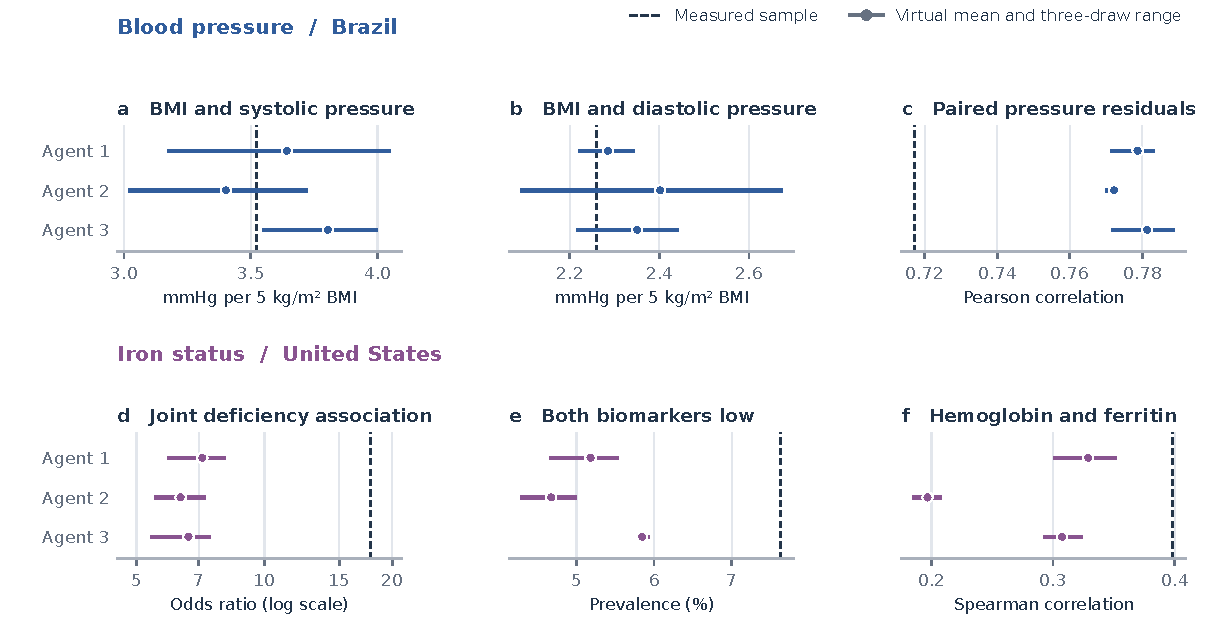
\includegraphics[width=.96\textwidth]{figures/original-paper.pdf}
\caption{The same analysis run on virtual and measured records. Each point is one constructor's mean across three seeded draws. The segment spans those draws. Dashed lines are measured sample estimates. Each panel has its own scale. The systolic slopes are near the Brazilian estimate. The iron odds ratios cluster around the value derived from the Chinese source paper, well below the US estimate.}
\Description{Six panels compare three constructors with a measured reference. The three systolic slopes straddle the reference, all diastolic slopes and residual correlations exceed it, and all three iron odds ratios, joint prevalences and rank correlations fall below their reference.}
\label{fig:original}
\end{figure*}

Table~\ref{tab:profile} preserves all three primary endpoints and the accompanying diagnostics in each case. Author numbers identify independent sessions within one task. The zero ordering violation rate follows from the positive pulse-pressure construction. Across the iron sessions, the two marginal deficiency fractions move in opposite directions relative to the US sample. The isolated threshold odds ratio is therefore an incomplete guide to biomedical utility.

\begin{table}[htbp]
\caption{All original-paper estimates. A1--A3 are constructor means over three seeded draws. The final column is the measured sample. Percentages use a 0--100 scale.}
\label{tab:profile}
\centering
\begin{tabular}{@{}lrrrr@{}}
\toprule
Analysis & A1 & A2 & A3 & Measured\\
\midrule
\multicolumn{5}{@{}l}{\emph{Brazilian blood pressure}}\\
BMI--SBP slope & 3.642 & 3.402 & 3.804 & 3.524\\
BMI--DBP slope & 2.285 & 2.402 & 2.350 & 2.260\\
Residual correlation & .779 & .772 & .781 & .717\\
SBP SD (mmHg) & 20.00 & 19.70 & 19.57 & 18.19\\
DBP SD (mmHg) & 11.57 & 11.57 & 11.47 & 11.09\\
SBP $<$ DBP (\%) & 0 & 0 & 0 & 0\\
\midrule
\multicolumn{5}{@{}l}{\emph{US iron status}}\\
Threshold odds ratio & 7.141 & 6.348 & 6.625 & 17.790\\
Both low (\%) & 5.180 & 4.673 & 5.847 & 7.630\\
Spearman correlation & .329 & .197 & .307 & .398\\
Low hemoglobin (\%) & 10.660 & 8.807 & 11.727 & 15.240\\
Low ferritin (\%) & 15.680 & 18.513 & 17.487 & 12.153\\
\bottomrule
\end{tabular}
\end{table}

\section{Two blood-pressure laws under the same constraints}
\label{app:laws}

\begin{figure*}[t]
\centering
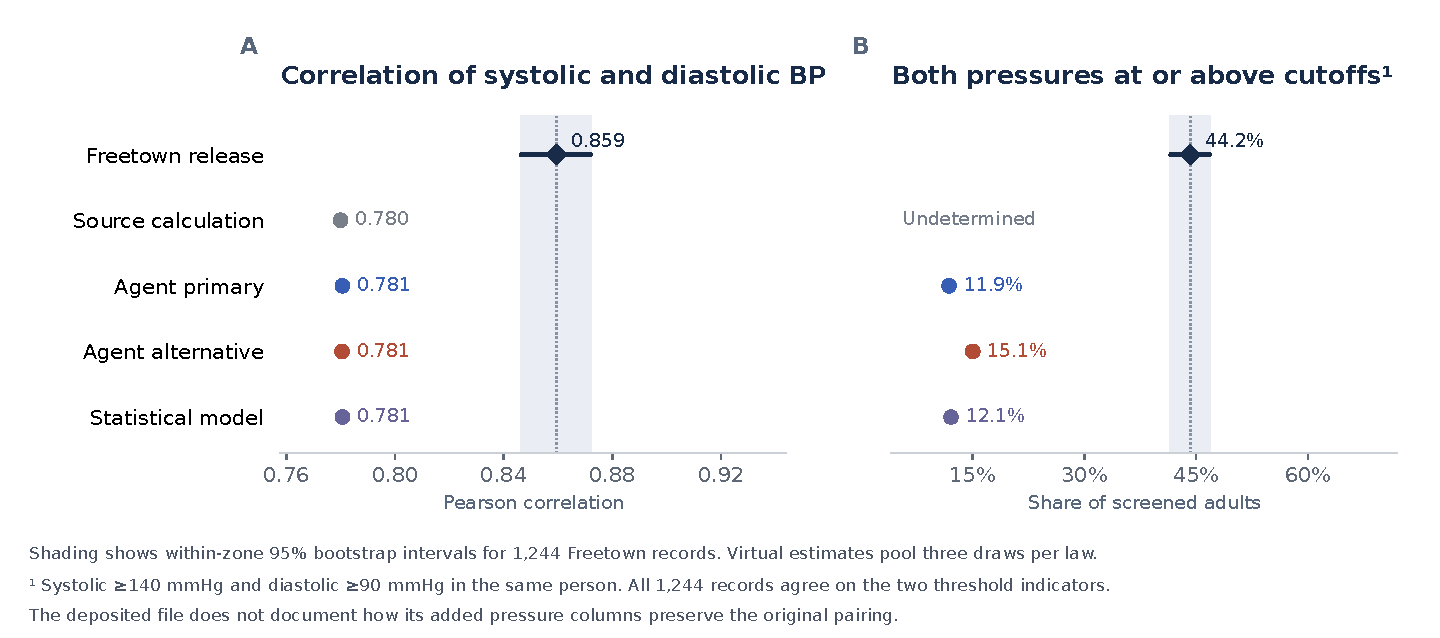
\includegraphics[width=.94\textwidth]{figures/freetown.pdf}
\caption{Prospective screening test. The source correlation is available by direct calculation. The joint threshold probability depends on the model. Points for the two agent laws and the statistical comparator are estimates from seeded virtual draws. The band describes uncertainty for the deposited Freetown sample conditional on the represented zones. The extreme target threshold result led to a separate audit of the deposited fields.}
\Description{Two panels show a released correlation of 0.859 and a joint threshold percentage of 44.2. Three virtual arms give correlations near 0.78 and threshold percentages between 11.9 and 15.1.}
\label{fig:freetown}
\end{figure*}

Let $S$ and $D$ be systolic and diastolic pressure. Write $G=S-D$ for the pulse-pressure gap. From the five source statistics, calculate
\begin{align*}
\mathrm{E}[G] &= \mathrm{E}[S]-\mathrm{E}[D],\\
\mathrm{Cov}(D,G) &= \mathrm{Cov}(S,D)-\mathrm{Var}(D),\\
\mathrm{Var}(G) &= \mathrm{Var}(S)+\mathrm{Var}(D)-2\mathrm{Cov}(S,D).
\end{align*}
The primary program draws positive $(D,G)$ from a bivariate lognormal distribution with these moments. For a vector of positive means $m$ and covariance $V$, the log covariance entries are $\log(1+V_{ij}/(m_i m_j))$ and the log means are $\log m_i$ minus half the corresponding log variance. Here the resulting matrices are positive definite. Setting $S=D+G$ enforces the intended ordering in every row.

The alternative program assigns probabilities 0.75 and 0.25 to components with means $(S,D)=(116.22,76.54)$ and $(152.22,92.54)$ mmHg. In $(D,G)$ coordinates, each component receives a common within-component covariance equal to the required total covariance minus the covariance of the component means. By the total covariance identity this gives the same unconditional first and second moments. The component probabilities and offsets are modeling choices. Conditional-normal quadrature for the event $\{D\geq90,\ D+G\geq140\}$ gives the probabilities in Section~\ref{sec:prospective}. Moments alone do not select either law.

\paragraph{Pre-disclosure design and measurement.}
The team screened eligibility, headers, uniqueness, measurement methods and field completeness before fixing the Freetown analysis. The target release identity and outcomes were withheld from the constructor. The primary, alternative, comparator, judgments and integration results were recorded before inspecting the measured joint outcomes. Construction took one recorded GPT call (US\$0.0845 at the recorded tariff). Each law generated three equal-sized draws of 10,000, including three for the independently implemented statistical comparator. The source protocol averaged the last two of three seated readings after at least 15 minutes' rest. Freetown averaged two readings following 3--5 minutes of rest. The source selected partnered rural adults, whereas the target was an urban community screening sample.

The Freetown reference uses paired positive recorded pressure values in prespecified age categories covering adults 40 and older. We computed an unweighted sample correlation and exceedance fraction. Intervals use 2,000 bootstraps of participants within eight zones, conditional on those zones. Across the full release, the audit counted 871 records meeting both thresholds, 1,523 meeting neither and zero in either discordant cell. These counts refer to deposited values. Field-level provenance would be needed to explain the pattern.



\section{Original-paper iron construction and verification}
\label{app:ironpros}

\begin{figure*}[t]
\centering
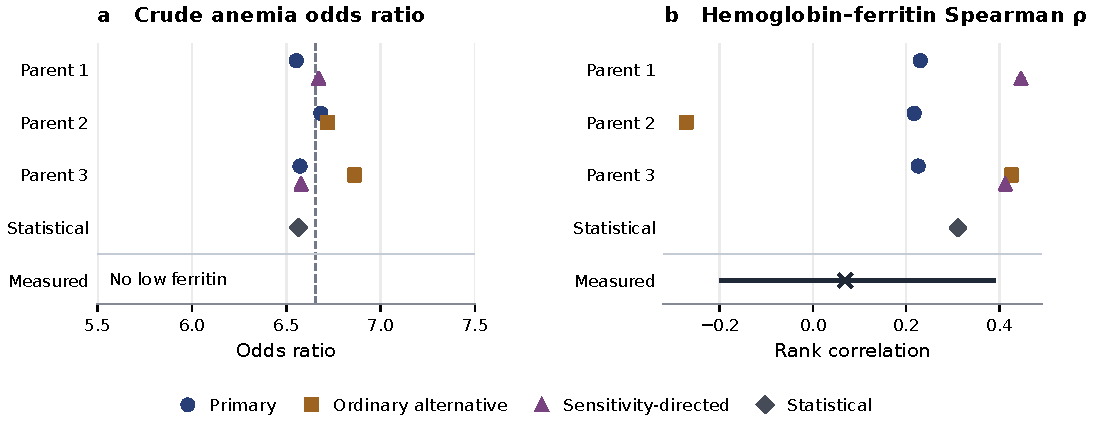
\includegraphics[width=.98\textwidth]{figures/iron-alternatives.pdf}
\caption{Two analyses on each sealed iron cohort. Symbols in each parent row distinguish the primary law and the two alternative requests. Two requests reached the output limit and have no point. The dashed line marks the source odds ratio of 6.65. The measured row gives the survey-weighted result for 44 women. The rank interval resamples villages within province. No woman in this sample had low measured ferritin.}
\Description{Agent odds ratios cluster between 6.55 and 6.86. Their rank correlations range from minus 0.272 to plus 0.446. The measured rank correlation is 0.069, with a wide interval.}
\label{fig:ironpros}
\end{figure*}

The protocol specified three independent primary sessions, two branches per primary, three seeds per executable law and 20,000 independent draws per seed. GPT-6.1 Sol received the original paper and a target description. It supplied the structure, parameters, prospective judgments and Python code. The statistical comparator used the same source and independent within-cell ranks. Two of nine requests (ordinary branch of parent 1, directed branch of parent 2) exhausted the 12,288-token output allowance. Usage across all nine requests cost an estimated US\$1.37 at the recorded tariff.

The original interface failed on all seven complete programs. Each program expected its named parameters at a different nesting level than the runner supplied. After the primary submissions were inspected and before simulated or measured outcomes were examined, we registered one mechanical rule to pass the nested parameter object following the same missing-key error on all three seeds. This rule preserved every scientific constant, line of sampler code, seed and target task. Original executions, failures and corrected executions were archived separately. The seven agent programs and one statistical program then produced 24 tables. All source assessments and model comparisons were committed before external disclosure.

The source checks cover four crude-cell frequencies, the crude log odds ratio, three hemoglobin-band frequencies, three ferritin-depletion fractions, three within-band ferritin geometric means, and both overall geometric means. These 16 checks overlap. Tolerances allow rounding, four estimated Monte Carlo standard errors and fixed operational allowances. Table~\ref{tab:ironprospective} gives the pooled simulated estimates. Each completed pair's absolute rank gap was 0.187--0.489. Subtracting its estimated 95\% Monte Carlo margin left 0.175--0.475. These margins describe simulation precision conditional on fixed laws.

\begin{table}[H]
\caption{Prospective iron analyses by parent and request. Each completed law contributes three draws. The last column records the complete source screen.}
\label{tab:ironprospective}
\centering
\begin{tabular}{@{}lrrl@{}}
\toprule
Construction & Odds ratio & Spearman $\rho$ & Screen\\
\midrule
P1 primary & 6.553 & 0.230 & pass\\
P1 ordinary & -- & -- & incomplete\\
P1 directed & 6.672 & 0.446 & pass\\
P2 primary & 6.683 & 0.217 & pass\\
P2 ordinary & 6.718 & -0.272 & pass\\
P2 directed & -- & -- & incomplete\\
P3 primary & 6.573 & 0.226 & pass\\
P3 ordinary & 6.862 & 0.426 & pass\\
P3 directed & 6.579 & 0.413 & pass\\
Statistical & 6.564 & 0.311 & pass\\
\bottomrule
\end{tabular}
\end{table}

\section{What can change while the selected iron summaries stay fixed?}
\label{app:ironproof}
Consider a single published hemoglobin band and ferritin-depletion cell with positive probability. Keep its probability and the two continuous conditional marginal distributions fixed. Draw hemoglobin from its conditional quantile function at a uniform rank $U$. One law draws ferritin from its conditional quantile at an independent uniform rank $V$. Another draws ferritin at $U$ with probability $\lambda>0$ and at $V$ otherwise. All other cells can stay fixed. The four threshold counts, each hemoglobin-band probability, and the ferritin geometric mean and depletion frequency in each band are invariant in the population. The overall geometric means are invariant as well.
For continuous marginal distributions, Spearman correlation is $12\,\mathbb{E}[F_H(H)F_F(F)]-3$. Within a nondegenerate cell the two marginal ranks are increasing functions of their corresponding uniforms. Sharing a uniform gives them positive covariance relative to independence. Hence the overall rank correlation changes while all the listed summaries remain fixed. This construction explains the ambiguity for the specified summaries. It supplies neither a biological estimate of the coupling nor its feasible range under additional evidence.

\section{Matched-size lifestyle analysis}
\label{app:lifestyle}

\begin{figure*}[t]
\centering
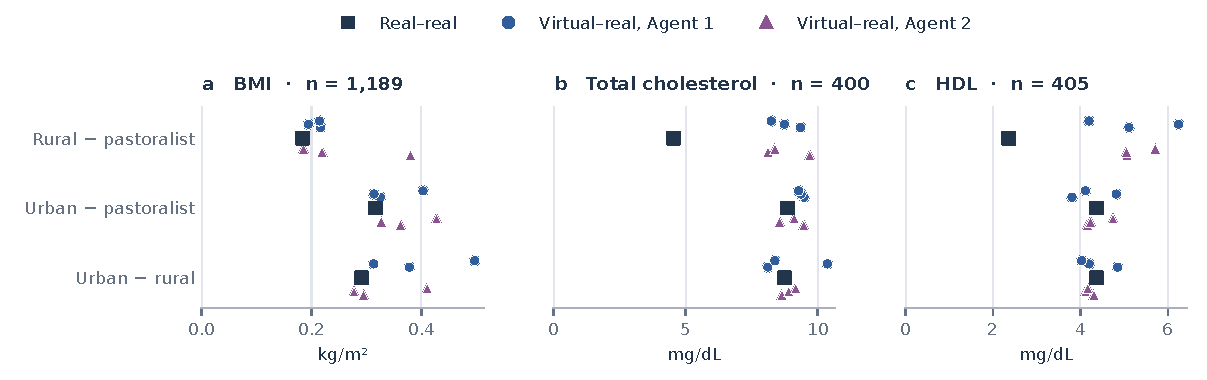
\includegraphics[width=.92\textwidth]{figures/lifestyle.pdf}
\caption{Matched-size mean absolute discrepancies for all nine adjusted lifestyle contrasts. The real--real estimate comes from two resamples of measured records. The virtual--real estimates use six saved virtual tables from two constructors. Native units and sample sizes differ across panels.}
\Description{Three panels compare BMI, total cholesterol and HDL across rural, urban and pastoralist lifestyles. Virtual versus real discrepancies are similar to real versus real for the urban BMI contrast, and larger for both rural lipid contrasts.}
\label{fig:lifestyle}
\end{figure*}

The original Turkana regression compared three lifestyle groups, adjusting each trait for age and sex~\cite{lea}. Real and virtual samples were matched on six sex-by-lifestyle stratum sizes within each trait. There were 1,189 eligible BMI measurements, 400 total cholesterol measurements and 405 HDL measurements. Each of 500 repetitions drew two real samples from the same empirical pool and one sample from each fixed virtual table. The virtual samples shared the second real sample as their reference. This design conditions on sample size, available cases and stratum counts. It leaves age and the outcomes free to vary. The bootstrap uses participants and does not model household or site clustering.



\begin{table*}[t]
\caption{Absolute discrepancies in matched-size lifestyle regressions. R and U denote rural and urban groups, and P denotes pastoralists. V--R gives the range across six fixed tables.}
\label{tab:lifestyle}
\centering
\begin{tabular}{@{}llrr@{}}
\toprule
Outcome & Contrast & Real--real & V--R\\
\midrule
BMI & R--P & .184 & .185--.380\\
(kg/m$^2$) & U--P & .316 & .314--.428\\
 & U--R & .291 & .277--.497\\
\midrule
Total cholesterol & R--P & 4.543 & 8.118--9.695\\
(mg/dL) & U--P & 8.848 & 8.556--9.479\\
 & U--R & 8.743 & 8.110--10.365\\
\midrule
HDL cholesterol & R--P & 2.363 & 4.195--6.242\\
(mg/dL) & U--P & 4.375 & 3.807--4.818\\
 & U--R & 4.362 & 4.029--4.851\\
\bottomrule
\end{tabular}
\end{table*}

Only 37 urban participants contributed total cholesterol measurements and 38 contributed HDL measurements. This small group helps explain the wide real--real variation. The discrepancy estimates in Table~\ref{tab:lifestyle} describe the observed composition. Equivalence for a planning decision would require a tolerance justified for that decision.

\section{Prospective external comparison in Akwa Ibom}
\label{app:akwa}
The Akwa Ibom study in southern Nigeria was second on the project's previously ordered list of iron cohorts. We screened the data dictionary, release terms, availability and uniqueness of participant keys before measuring either endpoint. Among the 1,290 biochemical records, 603 female participants in the mothers' group were aged 18--49 and had positive, finite Hb and serum ferritin. They came from 30 enumeration areas in 10 local government areas. The biochemical file supplies no analysis weight or pregnancy indicator. We report the sampled mothers' crude rank correlation and threshold odds using uncorrected ferritin. These characteristics limit transport from the Chinese cohorts. IITA and HarvestPlus supervised the original survey with support from the Bill \& Melinda Gates Foundation to HarvestPlus~\cite{akwa_iron}.

The article, aggregate supplement, task, seeds and hidden data digest were fixed before dispatch. The common virtual marginals came from the source-only CHNS A fit. Every law received the same sorted Hb and ferritin values in each of three Hb bands. The agent returned a sampler that assigns a permutation of ferritin values to the Hb values in each band, plus its parameters and their rationale. Six fresh sessions used the same GPT configuration. For the statistical arm we fit one Gaussian copula parameter to the supplied geometric-mean ferritin ratio of 1.215 comparing $13\leq\mathrm{Hb}<14$ with $12\leq\mathrm{Hb}<13$. Numerical integration gave a latent normal correlation of 0.137. The statistical law used this value in all three bands. Each law received the same three seeds and 12,000 virtual pairs per seed. Pairing preserves the threshold counts exactly across arms. The source ratio and each law's realized middle-band contrast remain available for checking.

We pooled each law's three draws for scoring and resampled whole enumeration areas within each local government area 2,000 times. Each paired bootstrap replicate compared all frozen laws with the same measured resample. Its interval describes sampling variation conditional on these particular constructors. The prespecified rule required at least four executable constructors, a median improvement of at least 0.02 in absolute rank error, a positive lower 95\% bound and a common threshold odds ratio within a factor of 1.50 of the measured odds ratio with at least ten observations per measured cell. Around a rank correlation of 0.30, the 0.02 margin corresponds to about a 13\% difference in an illustrative Fisher-transformation planning calculation.

\begin{table}[t]
\caption{Akwa Ibom external comparison. The middle-band ratio uses the two geometric mean ferritin levels defined above. The Chinese source ratio supplied to every constructor was 1.215.}
\label{tab:akwa}
\centering\small
\begin{tabular}{@{}lrrr@{}}
\toprule
Law or sample & Rank & Abs.\ rank error & Middle ratio\\
\midrule
Akwa Ibom sample & 0.0103 & --- & 0.9491\\
Statistical generator & 0.3031 & 0.2928 & 1.2254\\
Agent 1 & 0.3082 & 0.2979 & 1.2440\\
Agent 2 & 0.3082 & 0.2979 & 1.2440\\
Agent 3 & 0.3082 & 0.2979 & 1.2440\\
Agent 4 & 0.3082 & 0.2979 & 1.2439\\
Agent 5 & 0.3082 & 0.2979 & 1.2440\\
Agent 6 & 0.3082 & 0.2979 & 1.2440\\
\bottomrule
\end{tabular}
\end{table}

All six source programs and model responses had distinct hashes. At shared seeds five programs produced the same arrays, and the sixth produced slightly different arrays. The largest distance between any sealed agent rank and the statistical rank was 0.00509. By the reverse triangle inequality this also bounds the difference in their absolute errors for \emph{any} target rank. Consequently the 0.02 margin was already unattainable before disclosure. Both endpoints of the paired percentile interval rounded to $-0.00509$. Whenever the resampled reference rank falls below both estimates, it cancels from their paired error difference. The interval for the measured rank itself was much wider. This paired interval is conditional on the sealed laws and shared seeds. Table~\ref{tab:akwa} shows all constructions.

All four threshold cells in the measured sample contained at least 22 mothers. The common virtual odds ratio was 4.49 times the measured value, exceeding the 1.50 guard. The comparison preserves both virtual marginals in each band, so this discrepancy applies to both arms. Different source and target sampling frames, assays, inflammation and pregnancy status could influence transport. This experiment cannot assign the discrepancy to any one cause. The six calls cost an estimated US\$0.484 at the recorded tariff.

Independent scoring from the official Stata file reproduced the point estimates, the two measured intervals and the paired error interval. A check frozen before disclosure required identical ranks to $10^{-12}$ across the official Stata and text files. Text serialization merged the ranks of two ferritin readings. Its estimate differed by $4.32\times10^{-6}$, with the same threshold cells and decision. The separate code also checked all 21 virtual draws against their archived hashes and verified the two marginal multisets within every band.

\end{document}
